
\documentclass[letterpaper,hide notes,xcolor={table,svgnames},pdftex]{beamer}
\def\showexamples{t}


%\usepackage[svgnames]{xcolor}

%% Demo talk
%\documentclass[letterpaper,notes=show]{beamer}

\usecolortheme{crane}%seahorse crane
\setbeamertemplate{navigation symbols}{}

\usetheme{MyPittsburgh}
%\usetheme{Frankfurt}

%\usepackage{tipa}

\usepackage{hyperref}
\usepackage{graphicx,xspace}
\usepackage[normalem]{ulem}

\newcommand\SF[1]{$\bigstar$\footnote{SF: #1}}

\usepackage{paratype}
\renewcommand*\familydefault{\sfdefault} %% Only if the base font of the document is to be sans serif
\usepackage[zerostyle=c]{newtxtt}
\usepackage[T1]{fontenc}

\newcounter{tmpnumSlide}
\newcounter{tmpnumNote}

\usepackage{xcolor}
\usepackage{tabu}
\definecolor{light-gray}{gray}{0.75}
\taburulecolor{light-gray}

% old question code
%\newcommand\question[1]{{$\bigstar$ \small \onlySlide{2}{#1}}}
% \newcommand\nquestion[1]{\ifdefined \presentationonly \textcircled{?} \fi \note{\par{\Large \textbf{?}} #1}}
% \newcommand\nanswer[1]{\note{\par{\Large \textbf{A}} #1}}


 \newcommand\mnote[1]{%
   \addtocounter{tmpnumSlide}{1}
   \ifdefined\showcues {~\tiny\fbox{\arabic{tmpnumSlide}}}\fi
   \note{\setlength{\parskip}{1ex}\addtocounter{tmpnumNote}{1}\textbf{\Large \arabic{tmpnumNote}:} {#1\par}}}

\newcommand\mmnote[1]{\note{\setlength{\parskip}{1ex}#1\par}}

%\newcommand\mnote[2][]{\ifdefined\handoutwithnotes {~\tiny\fbox{#1}}\fi
% \note{\setlength{\parskip}{1ex}\textbf{\Large #1:} #2\par}}

%\newcommand\mnote[2][]{{\tiny\fbox{#1}} \note{\setlength{\parskip}{1ex}\textbf{\Large #1:} #2\par}}

\newcommand\mquestion[2]{{~\color{red}\fbox{?}}\note{\setlength{\parskip}{1ex}\par{\Large \textbf{?}} #1} \note{\setlength{\parskip}{1ex}\par{\Large \textbf{A}} #2\par}\ifdefined \presentationonly \pause \fi}

\newcommand\blackboard[1]{%
\ifdefined   \showblackboard
  {#1}
  \else {\begin{center} \fbox{\colorbox{blue!30}{%
         \begin{minipage}{.95\linewidth}%
           \hspace{\stretch{1}} Some space intentionally left blank; done at the blackboard.%
         \end{minipage}}}\end{center}}%
         \fi%
}



%\newcommand\q{\tikz \node[thick,color=black,shape=circle]{?};}
%\newcommand\q{\ifdefined \presentationonly \textcircled{?} \fi}

\usepackage{listings}
\lstset{%
  keywordstyle=\bfseries,
  aboveskip=15pt,
  belowskip=15pt,
  captionpos=b,
  identifierstyle=\ttfamily,
  escapeinside={(*@}{@*)},
  stringstyle=\ttfamiliy,
  frame=lines,
  numbers=left, basicstyle=\scriptsize, numberstyle=\tiny, stepnumber=0, numbersep=2pt}

\usepackage{siunitx}
\newcommand\sius[1]{\num[group-separator = {,}]{#1}\si{\micro\second}}
\newcommand\sims[1]{\num[group-separator = {,}]{#1}\si{\milli\second}}
\newcommand\sins[1]{\num[group-separator = {,}]{#1}\si{\nano\second}}
\sisetup{group-separator = {,}, group-digits = true}

%% -------------------- tikz --------------------
\usepackage{tikz}
\usetikzlibrary{positioning}
\usetikzlibrary{arrows,backgrounds,automata,decorations.shapes,decorations.pathmorphing,decorations.markings,decorations.text}

\tikzstyle{place}=[circle,draw=blue!50,fill=blue!20,thick, inner sep=0pt,minimum size=6mm]
\tikzstyle{transition}=[rectangle,draw=black!50,fill=black!20,thick, inner sep=0pt,minimum size=4mm]

\tikzstyle{block}=[rectangle,draw=black, thick, inner sep=5pt]
\tikzstyle{bullet}=[circle,draw=black, fill=black, thin, inner sep=2pt]

\tikzstyle{pre}=[<-,shorten <=1pt,>=stealth',semithick]
\tikzstyle{post}=[->,shorten >=1pt,>=stealth',semithick]
\tikzstyle{bi}=[<->,shorten >=1pt,shorten <=1pt, >=stealth',semithick]

\tikzstyle{mut}=[-,>=stealth',semithick]

\tikzstyle{treereset}=[dashed,->, shorten >=1pt,>=stealth',thin]

\usepackage{ifmtarg}
\usepackage{xifthen}
\makeatletter
% new counter to now which frame it is within the sequence
\newcounter{multiframecounter}
% initialize buffer for previously used frame title
\gdef\lastframetitle{\textit{undefined}}
% new environment for a multi-frame
\newenvironment{multiframe}[1][]{%
\ifthenelse{\isempty{#1}}{%
% if no frame title was set via optional parameter,
% only increase sequence counter by 1
\addtocounter{multiframecounter}{1}%
}{%
% new frame title has been provided, thus
% reset sequence counter to 1 and buffer frame title for later use
\setcounter{multiframecounter}{1}%
\gdef\lastframetitle{#1}%
}%
% start conventional frame environment and
% automatically set frame title followed by sequence counter
\begin{frame}%
\frametitle{\lastframetitle~{\normalfont(\arabic{multiframecounter})}}%
}{%
\end{frame}%
}
\makeatother

\makeatletter
\newdimen\tu@tmpa%
\newdimen\ydiffl%
\newdimen\xdiffl%
\newcommand\ydiff[2]{%
    \coordinate (tmpnamea) at (#1);%
    \coordinate (tmpnameb) at (#2);%
    \pgfextracty{\tu@tmpa}{\pgfpointanchor{tmpnamea}{center}}%
    \pgfextracty{\ydiffl}{\pgfpointanchor{tmpnameb}{center}}%
    \advance\ydiffl by -\tu@tmpa%
}
\newcommand\xdiff[2]{%
    \coordinate (tmpnamea) at (#1);%
    \coordinate (tmpnameb) at (#2);%
    \pgfextractx{\tu@tmpa}{\pgfpointanchor{tmpnamea}{center}}%
    \pgfextractx{\xdiffl}{\pgfpointanchor{tmpnameb}{center}}%
    \advance\xdiffl by -\tu@tmpa%
}
\makeatother
\newcommand{\copyrightbox}[3][r]{%
\begin{tikzpicture}%
\node[inner sep=0pt,minimum size=2em](ciimage){#2};
\usefont{OT1}{phv}{n}{n}\fontsize{4}{4}\selectfont
\ydiff{ciimage.south}{ciimage.north}
\xdiff{ciimage.west}{ciimage.east}
\ifthenelse{\equal{#1}{r}}{%
\node[inner sep=0pt,right=1ex of ciimage.south east,anchor=north west,rotate=90]%
{\raggedleft\color{black!50}\parbox{\the\ydiffl}{\raggedright{}#3}};%
}{%
\ifthenelse{\equal{#1}{l}}{%
\node[inner sep=0pt,right=1ex of ciimage.south west,anchor=south west,rotate=90]%
{\raggedleft\color{black!50}\parbox{\the\ydiffl}{\raggedright{}#3}};%
}{%
\node[inner sep=0pt,below=1ex of ciimage.south west,anchor=north west]%
{\raggedleft\color{black!50}\parbox{\the\xdiffl}{\raggedright{}#3}};%
}
}
\end{tikzpicture}
}


%% --------------------

%\usepackage[excludeor]{everyhook}
%\PushPreHook{par}{\setbox0=\lastbox\llap{MUH}}\box0}

%\vspace*{\stretch{1}

%\setbox0=\lastbox \llap{\textbullet\enskip}\box0}

\setlength{\parskip}{\fill}

\newcommand\noskips{\setlength{\parskip}{1ex}}
\newcommand\doskips{\setlength{\parskip}{\fill}}

\newcommand\xx{\par\vspace*{\stretch{1}}\par}
\newcommand\xxs{\par\vspace*{2ex}\par}
\newcommand\tuple[1]{\langle #1 \rangle}
\newcommand\code[1]{{\sf \footnotesize #1}}
\newcommand\ex[1]{\uline{Example:} \ifdefined \presentationonly \pause \fi
  \ifdefined\showexamples#1\xspace\else{\uline{\hspace*{2cm}}}\fi}

\newcommand\ceil[1]{\lceil #1 \rceil}


\AtBeginSection[]
{
   \begin{frame}
       \frametitle{Outline}
       \tableofcontents[currentsection]
   \end{frame}
}



\pgfdeclarelayer{edgelayer}
\pgfdeclarelayer{nodelayer}
\pgfsetlayers{edgelayer,nodelayer,main}

\tikzstyle{none}=[inner sep=0pt]
\tikzstyle{rn}=[circle,fill=Red,draw=Black,line width=0.8 pt]
\tikzstyle{gn}=[circle,fill=Lime,draw=Black,line width=0.8 pt]
\tikzstyle{yn}=[circle,fill=Yellow,draw=Black,line width=0.8 pt]
\tikzstyle{empty}=[circle,fill=White,draw=Black]
\tikzstyle{bw} = [rectangle, draw, fill=blue!20, 
    text width=4em, text centered, rounded corners, minimum height=2em]
    
    \newcommand{\CcNote}[1]{% longname
	This work is licensed under the \textit{Creative Commons #1 3.0 License}.%
}
\newcommand{\CcImageBy}[1]{%
	\includegraphics[scale=#1]{creative_commons/cc_by_30.pdf}%
}
\newcommand{\CcImageSa}[1]{%
	\includegraphics[scale=#1]{creative_commons/cc_sa_30.pdf}%
}
\newcommand{\CcImageNc}[1]{%
	\includegraphics[scale=#1]{creative_commons/cc_nc_30.pdf}%
}
\newcommand{\CcGroupBySa}[2]{% zoom, gap
	\CcImageBy{#1}\hspace*{#2}\CcImageNc{#1}\hspace*{#2}\CcImageSa{#1}%
}
\newcommand{\CcLongnameByNcSa}{Attribution-NonCommercial-ShareAlike}


\newenvironment{changemargin}[1]{% 
  \begin{list}{}{% 
    \setlength{\topsep}{0pt}% 
    \setlength{\leftmargin}{#1}% 
    \setlength{\rightmargin}{1em}
    \setlength{\listparindent}{\parindent}% 
    \setlength{\itemindent}{\parindent}% 
    \setlength{\parsep}{\parskip}% 
  }% 
  \item[]}{\end{list}} 




\title{Lecture 29 --- Collections}

\author{J. Zarnett\\
\texttt{jzarnett@uwaterloo.ca}}
\institute{Department of Electrical and Computer Engineering \\
  University of Waterloo}
\date{\today}

\begin{document}

\begin{frame}
  \titlepage
  
  \begin{center}
  \small{Acknowledgments: D.W. Harder, W.D. Bishop}
  \end{center}
\end{frame}

\begin{frame}
\frametitle{Collections}

Collections are groupings of some variable number of data elements.

Each collection type implements a data structure and the algorithms associated with the data structure.

We're going to examine the following collections:

\begin{itemize}
	\item List
	\item Stack
	\item Queue
\end{itemize}

Each of these collections may contain an arbitrary number of items.\\
\quad Although in practice, computer memory is not infinite.

\end{frame}

\begin{frame}
\frametitle{List}

We are all certainly familiar with the concept of a list.\\
\quad The ``to-do list'' of tasks to complete is a very common example:
\begin{itemize}
	\item Wash dishes
	\item Pick up dry cleaning
	\item Study for the final exam
\end{itemize}

The list may contain an arbitrary number of items and there is some concept of ordering: ``wash dishes'' is the first item in this list.

We can look at or access any item in the list.\\
\quad There's no rule that mandates washing the dishes before studying.

We can insert items anywhere in the list.\\
\quad Though the usual case is to add them at the end of the list.

\end{frame}


\begin{frame}
\frametitle{List}

The \alert{list} is a finite, ordered collection of values, in which repeated values are permitted. A list of integers, for example: \{4, 19, 756, 4, 18\}

The first object in the list is at the \textit{front} of the list; the last element is at the \textit{back} of the list.

A list supports several conceptual operations:
\begin{itemize}
	\item Access the $k^{th}$ element of the list
	\item Given a reference to an element of the list:
	\begin{itemize}
	\item Access the next or previous element
	\item Modify the current element
	\item Remove the current element
	\item Insert an element immediately before or after the current element
	\end{itemize}
\end{itemize}

\end{frame}


\begin{frame}
\frametitle{Working with the List}
On a list of integers \{4, 19, 756, 4, 18\}, let's perform some operations.

Add 42 to the end of the list: \\ \{4, 19, 756, 4, 18, 42\}

Remove 19 from the list: \\ \{4, 756, 4, 18, 42\}

Insert 99 before 756: \\ \{4, 99, 756, 4, 18, 42\}

\end{frame}

\begin{frame}
\frametitle{The Stack and Queue}
The \alert{stack} and \alert{queue} are also collections like a list, but with restrictions on how elements may be accessed, added, or removed.

A stack has a last-in, first-out policy: the only element that may be removed from the collection is the one most recently added.

A queue has first-in, first-out behaviour: the only element that may be removed is the one that has been in the queue the longest.

\end{frame}

\begin{frame}
\frametitle{The Stack and Queue}

\vspace{3em}

\begin{columns}
\begin{column}{.48\textwidth}
\begin{center}
\underline{\textbf{Stack}}
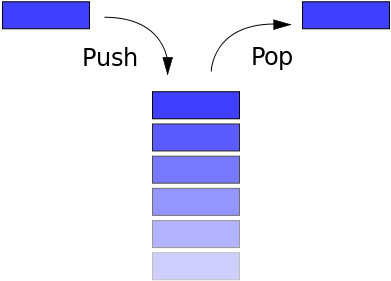
\includegraphics[width=\textwidth]{images/data_stack.png}\\
{\tiny Image source: Shrimp/Wikipedia\\
 \url{http://upload.wikimedia.org/wikipedia/commons/2/29/Data_stack.svg}}
\end{center}
\end{column}

\begin{column}{.48\textwidth}
\begin{center}
\underline{\textbf{Queue}}
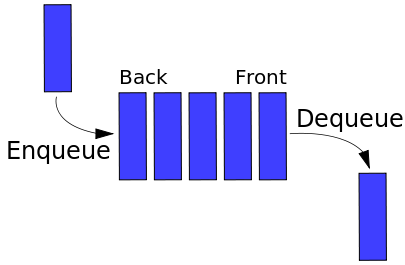
\includegraphics[width=\textwidth]{images/data_queue.png}\\
{\tiny Image source: Vegpuff/Wikipedia\\
 \url{http://upload.wikimedia.org/wikipedia/commons/5/52/Data_Queue.svg}}

\end{center}
\end{column}
\end{columns}

\end{frame}


\begin{frame}
\frametitle{Stack}
We have already introduced the stack when discussing memory.\\
Recall: the stack as a series of boxes piled one on top of another.

Let's continue that stacked boxes example:\\
\quad The box at the top is the only one you can use.\\
\quad When finished with a box, you take it off the top of the pile.\\
\quad Any new box to be added goes on top of the pile.\\
\quad It's not possible to take a box out of the middle.

\end{frame}


\begin{frame}
\frametitle{Stack}

The stack conceptually supports 3 operations: \alert{push}, \alert{peek}, and \alert{pop}.

Push adds an element to the top of the stack.\\
Peek examines the element at the top of the stack.\\
Pop removes and returns the element at the top of the stack.

Note that peek does not remove the element at the top of the stack.

If we attempt to pop when there are no items on the stack, the result is an error called \textit{stack underflow}.

If we attempt to push an item when there is no more space in the underlying representation, the result is a \textit{stack overflow} error.

\end{frame}

\begin{frame}
\frametitle{Working with the Stack}
On the board, let's visualize how the stack works conceptually for the following sequence of operations. We start with an empty stack.

\begin{enumerate}
	\item Push 74
	\item Peek
	\item Push 867
	\item Push 97
	\item Peek
	\item Pop
	\item Push 44
	\item Peek
	\item Pop
	\item Pop
	\item Pop
	\item Pop
\end{enumerate}


\end{frame}


\begin{frame}
\frametitle{Queue}

You've surely spent plenty of time in queues over the years.\\
\quad In common speech, we typically use the word ``line''.\\
\quad When you have to wait in a line for your turn, you are in a queue.


Example: waiting to order at a fast food restaurant.\\

\quad The customer at the front of the line is the next one served.\\
\quad Then the line moves up and someone else is at the front of the line.\\
\quad When a new customer arrives, s/he goes to the back of the line.\\
\quad Cutting in line (going out of turn) is not permitted.

\end{frame}


\begin{frame}
\frametitle{Queue}

The queue also supports 3 operations: \alert{enqueue}, \alert{peek}, and \alert{dequeue}.

Enqueue adds an element to the end of the queue.\\
Peek examines the element at the front of the queue.\\
Dequeue removes and returns the element at the front of the queue.

Peek does not remove the element at the front of the queue.

If we attempt to dequeue when there are no items on the stack, the result is an error called \textit{queue underflow}.

If we attempt to enqueue an item when there is no more space in the underlying representation, the result is a \textit{queue overflow} error.

\end{frame}

\begin{frame}
\frametitle{Working with the Queue}
On the board, let's visualize the same sequence but for a queue. Again, starting with an empty queue.

\begin{enumerate}
	\item Enqueue 74
	\item Peek
	\item Enqueue 867
	\item Enqueue 97
	\item Peek
	\item Dequeue
	\item Enqueue 44
	\item Peek
	\item Dequeue
	\item Dequeue
	\item Dequeue
	\item Dequeue
\end{enumerate}


\end{frame}


\begin{frame}
\frametitle{List and Array}
An array is very much like a list, although it is of fixed length. It has an ordering (the index), allows random access, insertion etc.

Arrays can be used to implement a list (although we will have to do resizing if the array gets full).

An array can also be used to implement a stack or queue.\\
\quad You will get a chance to implement this in ECE~250.

For now, we won't write our own implementations of the collections.

Now that you are familiar with how they work conceptually, let us examine one of the built-in collections.

\end{frame}


\begin{frame}
\frametitle{The \texttt{ArrayList}}

The C\# collection we will examine is the: \texttt{ArrayList}.

The \texttt{ArrayList} class models a list and behaves like an array:\\
\quad The index operators may be used to access array elements; but \\
\quad Elements are added using an \texttt{Add( )} method provided by the class.

It is important to note that the type of objects added to the ArrayList class is not specified directly. Any type can be put in the collection.
\end{frame}

\begin{frame}[fragile]
\frametitle{Using \texttt{ArrayList}}
{\scriptsize
\begin{verbatim}
ArrayList people = new ArrayList(3);
		
people.Add( "Bill" );
people.Add( "George" );
people.Add( "Dave" );

foreach( string s in people )
{
    Console.WriteLine( s );
}
Console.Write( "\n" );

people.Add( "Faye" );
people.Add( "Jason" );
people.Add( "David" );
people.Add( "Matt" );
people.Add( "Zac" );

foreach( string s in people )
{
    Console.WriteLine( s );
}
Console.Write( "\n" );
\end{verbatim}
}
\end{frame}


\begin{frame}
\frametitle{Using \texttt{ArrayList}}

Every time we call \texttt{Add( )}, we put the new element in the list, after the last already-present element.

Even though we initialized the \texttt{ArrayList} with a capacity of 3, we were able to add 5 more elements to the list.

The collection increases its own capacity dynamically when items are added beyond its current capacity.

\end{frame}

\begin{frame}
\frametitle{Methods Provided by \texttt{ArrayList}}
Don't attempt to memorize this, but the following table outlines the built-in methods of the \texttt{ArrayList} class that you may find useful:

{\scriptsize
\begin{center}
\begin{tabular}{p{4.4cm}|p{6.25cm}}
	\textbf{Method} & \textbf{Description} \\ \hline
	int Add( Object v ) & Adds v to an instance of the ArrayList class and returns the index of the object position in the ArrayList\\ \hline
void AddRange( ICollection c ) & Adds a collection of objects named c to an instance of the ArrayList class\\ \hline
int BinarySearch(Object v )& Searches an instance of an ArrayList class for v and returns the index of the object position in the ArrayList\\ \hline
void Clear( ) & Clears an instance of an ArrayList class but maintains its maximum capacity\\ \hline
int IndexOf( Object v ) & Returns the first index of v in an instance of an ArrayList class\\ \hline
void Insert( int i, Object v ) & Inserts v at index i to an instance of the ArrayList class\\ \hline
void InsertRange( int i, {ICollection} c ) & Inserts a collection of objects named c at index i to an instance of the ArrayList class\\ \hline
int LastIndexOf(Object v ) & Returns the last index of an object v in array a\\ \hline
void Sort( ) & Sorts an array named a\\ \hline
object[] ToArray( ) & Converts an instance of an ArrayList class to an array
\end{tabular}
\end{center}
}

\end{frame}

\begin{frame}[fragile]
\frametitle{Concatenation with \texttt{ArrayList}}
{\scriptsize
\begin{verbatim}
ArrayList people = new ArrayList(3);
people.Add( "Bill" );
people.Add( "George" );
people.Add( "Dave" );

ArrayList people2 = new ArrayList(5);
people2.Add( "Faye" );
people2.Add( "Jason" );
people2.Add( "David" );
people2.Add( "Matt" );
people2.Add( "Zac" );

people.AddRange( people2 );

foreach( string s in people )
{
    Console.WriteLine( s );
}
Console.Write( "\n" );
\end{verbatim}
}
\end{frame}



\begin{frame}
\frametitle{Internals of the \texttt{ArrayList}}

The internal structure of the \texttt{ArrayList} class is not documented, and could therefore change in any update of the C\# framework.

However, the following information is known about the \texttt{ArrayList}:
\begin{itemize}
\item Instances of \texttt{ArrayList} have a fixed capacity set at the time of object construction
\item The capacity defaults to 16 objects
\item The capacity of the \texttt{ArrayList} may be modified using the Capacity property
\item The capacity of the \texttt{ArrayList} is automatically doubled whenever object(s) are inserted and the existing capacity is insufficient
\end{itemize}

\end{frame}

\begin{frame}
\frametitle{Behind the Scenes of \texttt{ArrayList}}
As the name says, the \texttt{ArrayList} is a list implemented as an array.

It will resize itself as necessary, but because it is based on an array, the resizing will involve copying the elements to a bigger array.

So it is built-in implementation of the array resizing technique we saw previously, with the exact details hidden from us.

Next time, we'll look at building our own dynamic collection that truly has no arrays in it: the \alert{linked list}.

\end{frame}

\end{document}

